% -*- compile-command: "make HOCKING-slides.pdf" -*-
\documentclass{beamer}
\usepackage{tikz}
\usepackage[all]{xy}
\usepackage{amsmath,amssymb}
\usepackage{hyperref}
\usepackage{graphicx}
\usepackage{algorithmic}

\DeclareMathOperator*{\argmin}{arg\,min}
\DeclareMathOperator*{\Lik}{Lik}
\DeclareMathOperator*{\Peaks}{Peaks}
\DeclareMathOperator*{\Segments}{Segments}
\DeclareMathOperator*{\argmax}{arg\,max}
\DeclareMathOperator*{\maximize}{maximize}
\DeclareMathOperator*{\minimize}{minimize}
\newcommand{\sign}{\operatorname{sign}}
\newcommand{\RR}{\mathbb R}
\newcommand{\ZZ}{\mathbb Z}
\newcommand{\NN}{\mathbb N}

\begin{document}

\title{Statistical machine 
learning algorithms for 
understanding big data in
  genomics and medicine}

\author{
  Toby Dylan Hocking\\
  toby.hocking@mail.mcgill.ca
}

\maketitle

\begin{frame}
  \frametitle{Toby Dylan Hocking, brief CV}
  \begin{description}
  \item[2002-2006] UC Berkeley, double major in Molecular Cell Biology
    and Statistics (honors thesis with Terry Speed).
  \item[2006-2008] Biochemistry and Statistics at Sangamo BioSciences.
  \item[2008-2009] Masters in Statistics, Paris 6.
  \item[2009-2012] PhD in Mathematics from Ecole Normale Superieure de
    Cachan, machine learning for cancer genomics with JP Vert (Inst Curie)
    and Francis Bach (INRIA).
  \item[2013] Postdoc in Computer Science (machine learning) with Masashi Sugiyama at Tokyo
    Institute of Technology.
  \item[2014-2017] Postdoc on machine learning for epigenomics
    at McGill with Guillaume Bourque.
  \end{description}
\end{frame}

\begin{frame}
  \frametitle{Labeling enables supervised machine learning algorithms}
  \begin{tabular}{ccc}
    Input: Photos & Cell images & Copy number profiles \\
    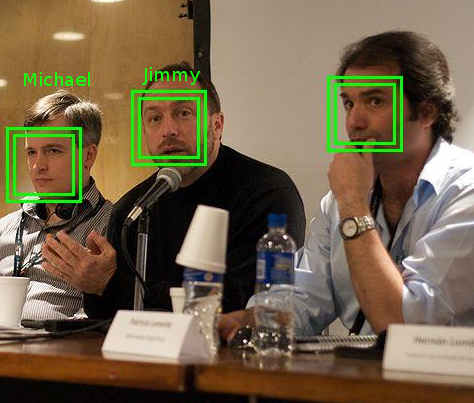
\includegraphics[width=1.3in]{faces} &
    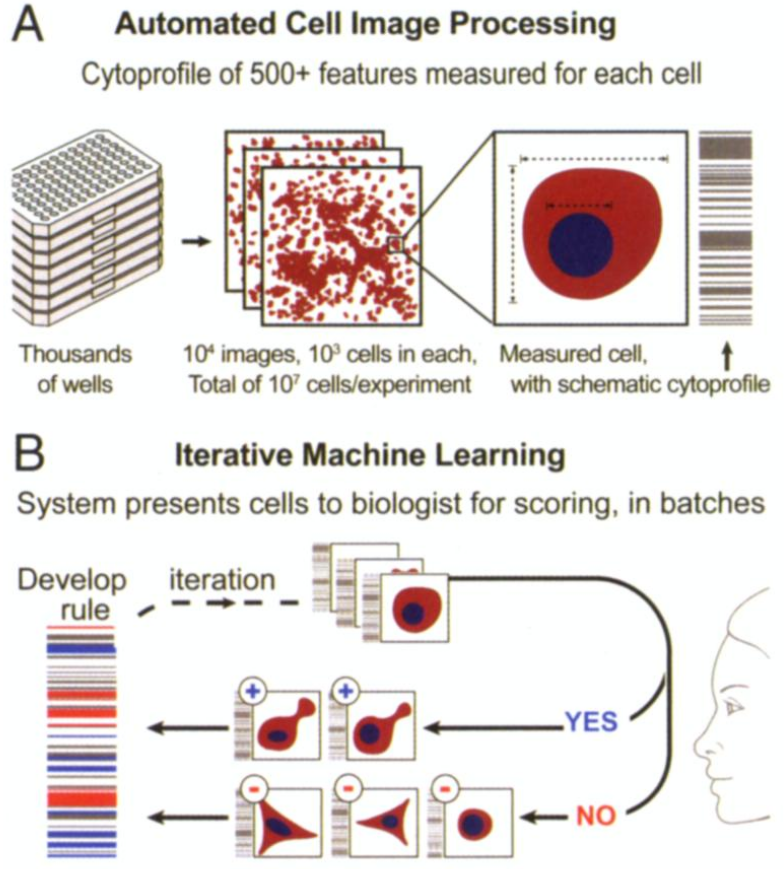
\includegraphics[width=1.3in]{cellprofiler} &
    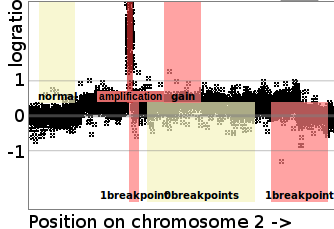
\includegraphics[width=1.5in]{regions-axes}\\
    Labels: boxes, names & phenotypes & alterations \\ \\
    %CVPR 2013
CVPR 2017
 & CellProfiler & SegAnnDB \\
    %246 papers
783 papers
 & 
%873 citations
1980 citations
 & H {\it et al.}, 2014. \\
     &
  \end{tabular}
  Sources: \url{http://en.wikipedia.org/wiki/Face_detection}\\
  Jones {\it et al.} PNAS 2009. Scoring diverse cellular morphologies in
  image-based screens with iterative feedback and machine learning.
\end{frame}

\begin{frame}
  \frametitle{Machine learning in computer vision and biology}
  ML is all about learning predictive functions $f(x)\approx y$, where 
  \begin{itemize}
  \item inputs/features $x$ are numerous (e.g. pixels or SNPs).
  \item outputs/labels $y$ are what we want to predict (typically
    phenotypes/classes).
  \item Input $x$ = image of digit,
    output $y\in\{0,1,\dots,9\}$,\\
  $f(
\includegraphics[height=1cm]{mnist-0})=0$,
  $f(
\includegraphics[height=1cm]{mnist-1})=1$
  % \item Input $x$ = image of article of clothing,\\
  %   output $y\in\{\text{shoe}, \text{pants}, \dots\}$,\\
  % $f(
\includegraphics[height=1cm]{fashion-mnist-boot})=\text{shoe}$,
  % $f(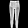
\includegraphics[height=1cm]{fashion-mnist-pants})=\text{pants}$
  \item Input $x$ = image of cell, 
    output $y\in\{\text{yes}, \text{no}\}$,\\
  $f(
\includegraphics[height=1cm]{cellprofiler-yes})=\text{yes}$,
  $f(
\includegraphics[height=1cm]{cellprofiler-no})=\text{no}$
  \item Input $x$ = genomic profile, output $y\in\{\text{breakpoint}, \text{normal}\}$
  $f(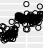
\includegraphics[height=1cm]{neuroblastoma-changepoint})=\text{breakpoint}$,
  $f(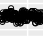
\includegraphics[height=1cm]{neuroblastoma-nochange})=\text{normal}$
  \end{itemize}
\end{frame}

\begin{frame}
  \frametitle{Unsupervised algorithms inaccurate for 
    complex patterns}
  \begin{itemize}
  \item Domain expert (biologist?) with prior knowledge manually codes an
    algorithm that recognizes the pattern.
  \item ``if the image $x$ has a dividing cell then predict
    $f(x)=\text{yes}$.''\\
    -- how to code that?
  \item ``if the copy number profile $x$ has a significant change of
    at least p-value $P$ in bins of size $B$, then predict
    $f(x)=\text{breakpoint}$.''\\
    -- sub-optimal parameter choices are inevitable.
    \end{itemize}
Disadvantages:
\begin{itemize}
  \item Need to find someone with programming experience AND domain expertise!
  \item Inaccurate: hard/impossible to manually write code that
    accurately recognizes complex patterns.
  \item Need to write a different algorithm for each pattern (0, 1, 2,
    %shoe, pants, 
    dividing cell, 
    normal cell,
    etc).
  \end{itemize}
\end{frame}

\begin{frame}
  \frametitle{Supervised machine learning }

  \begin{itemize}
  \item Domain expert labels examples using prior knowledge.
  \item Supervised algorithm learns $f$ based on labeled training data.
  \item State-of-the-art accuracy (if there is enough training data).
  \item Can use same learning algorithm regardless of pattern.
  \end{itemize}

  \begin{tabular}{cc}
  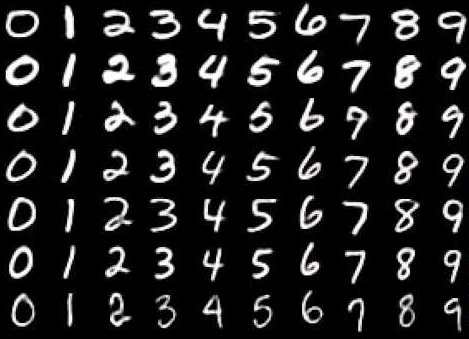
\includegraphics[height=1in]{mnist-digits} &
  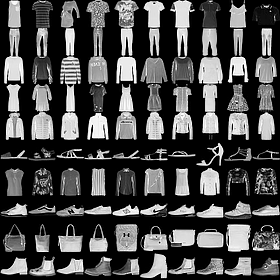
\includegraphics[height=1in]{fashion-mnist-sprite-some}  
  \end{tabular}

  \scriptsize Sources: github.com/cazala/mnist, github.com/zalandoresearch/fashion-mnist

  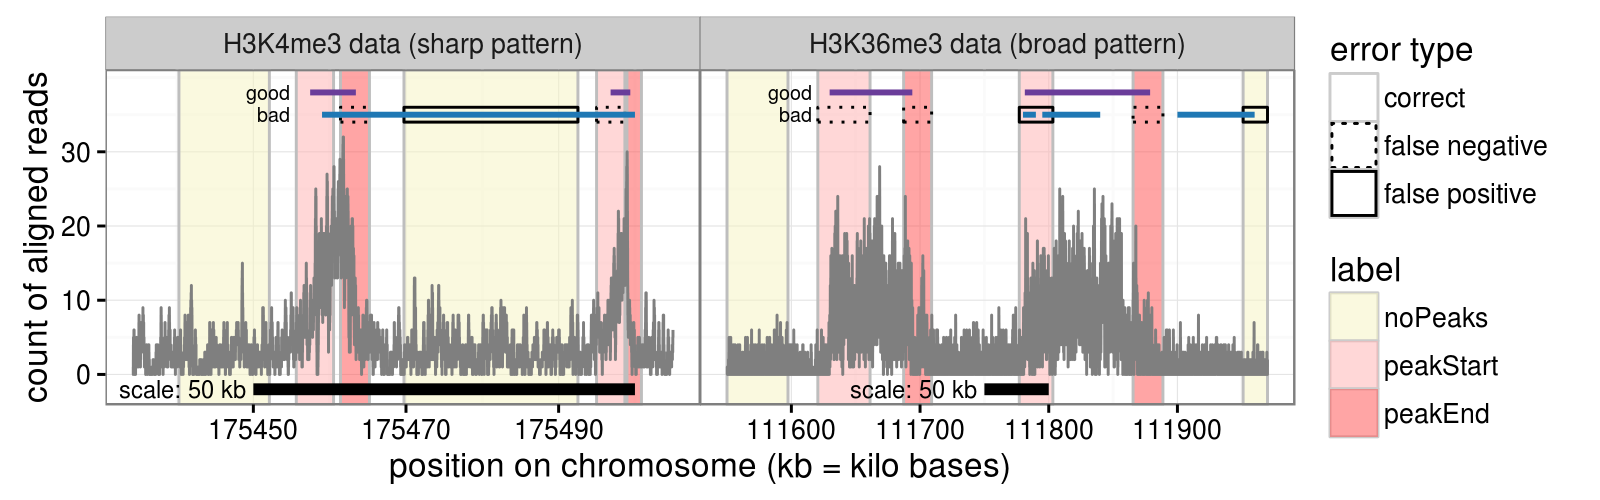
\includegraphics[width=\textwidth]{figure-good-bad}
\end{frame}

\begin{frame}
  \frametitle{My main research directions}
  Machine learning papers:
  \begin{itemize}
  \item How to learn $f$ which is as accurate as possible?
%\\ Mathematical optimization.
  \item How many labeled examples are required?
    %Statistics.\\
  \item Fast algorithms that scale linearly to huge data sets?
  \end{itemize}
  Bioinformatics papers:
  \begin{itemize}
  \item New labeling methods so we can use supervised machine learning
    algorithms for genomics/medicine.
  \item Algorithms that are fast enough for interactive labeling.
  \end{itemize}
  Applications papers (collaborations):
  \begin{itemize}
  \item What have we learned about the biology? (human learning)
  \end{itemize}
\end{frame}

\begin{frame}
  \frametitle{DNA COPY NUMBER ANALYSIS}
\end{frame}

\begin{frame}
  \frametitle{Cancer cells show chromosomal copy number alterations}
  Spectral karyotypes show the number of copies of the sex chromosomes
  (X,Y) and autosomes (1-22). 

  Source: Alberts \emph{et al.} 2002.
\vskip 0.1in
  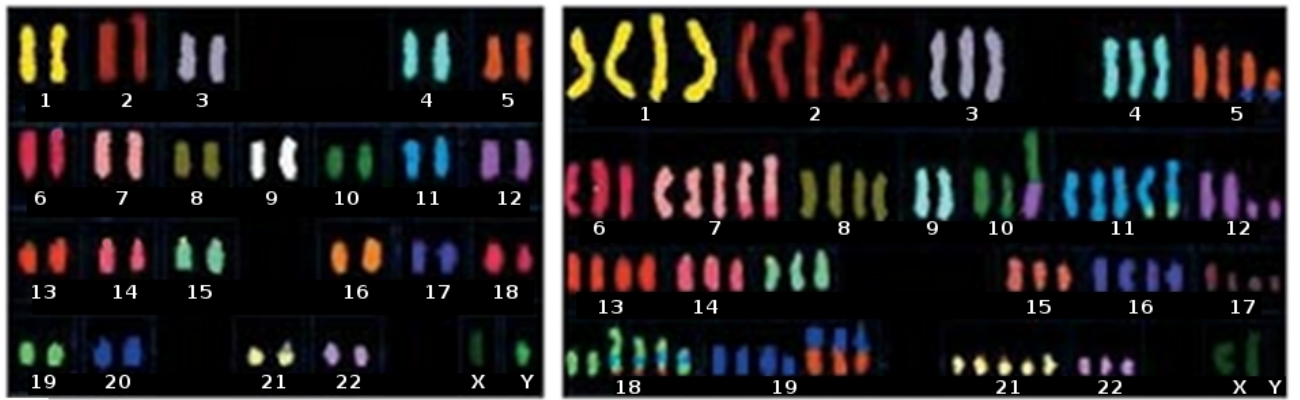
\includegraphics[width=\textwidth]{Karyo-both}
\vskip 0.1in
  \begin{minipage}{0.4\linewidth}
    Normal cell with 2 copies of each autosome.
  \end{minipage}
\hskip 0.1\linewidth
  \begin{minipage}{0.4\linewidth}
Cancer cell with many copy number alterations.
  \end{minipage}
\end{frame}

\begin{frame}
  \frametitle{Breakpoint detection is important in cancers such as
    neuroblastoma }

  \begin{itemize}
  \item Childhood cancer, most frequently diagnosed at age 1--2.
  \item Top three profiles ``ok'' -- no tumors after initial treatment.
  \item Bottom three ``relapse'' -- aggressive tumor within 5 years.
  \item Previous work: relapse profiles tend to have more breakpoints
     (Schleiermacher {\it et al.}, 2010).
  \end{itemize}

  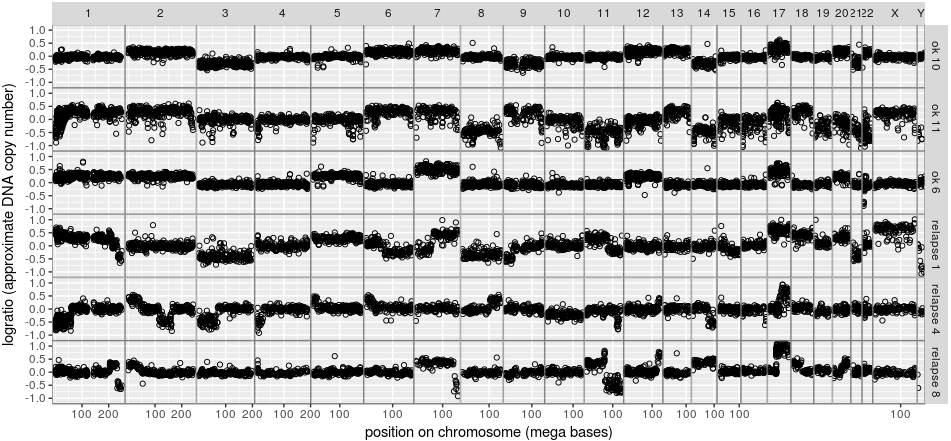
\includegraphics[width=\textwidth]{neuroblastoma-ok-relapse}
\end{frame}

\begin{frame}
  \frametitle{New labeling and training methods for breakpoint detection}

  H {\it et al.}, {\it BMC Bioinformatics} 2013.
  \begin{itemize}
  \item Benchmark data set of 3418 labeled chromosomes.
  \item Supervised training method: choose scalar significance parameter with
    minimal incorrect labels.
  \item Results: most accurate model is maximum likelihood Gaussian
    changepoint detection (K-fold cross-validation experiments).
  \end{itemize}

  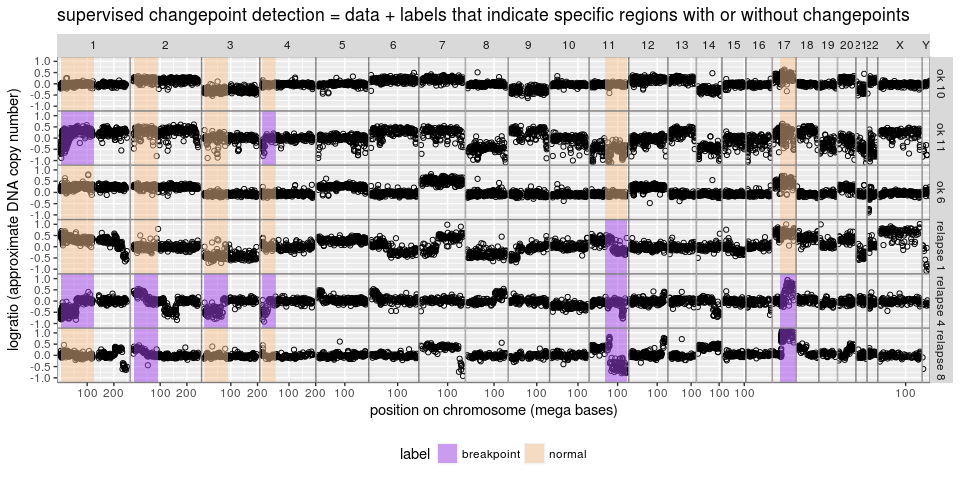
\includegraphics[width=\textwidth]{neuroblastoma-ok-relapse-supervised}

\end{frame}

\begin{frame}
  \frametitle{Supervised interactive DNA copy number analysis}
  H {\it et al.}, {\it Bioinformatics} 2014.

  \begin{itemize}
  \item Previous work: non-interactive command line programs
    -- collaborators can not correct obvious
    errors.
  \item Interactive system: when you edit the labels, the system
    learns and updates the model.
  \item Result: only a few labels required to learn a highly accurate
    breakpoint detection model.
  \end{itemize}

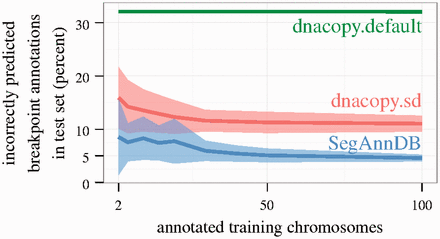
\includegraphics[width=0.5\textwidth]{SegAnnDB-test-error-decreases}

SegAnnDB demo: interactively label chr1 and chrX
  \url{http://bioviz.rocq.inria.fr/profile/GSM313887/}
\end{frame}

\begin{frame}
  \frametitle{Cancer biology collaborations}
  Aichi cancer center, Nagoya, Japan.
  \begin{itemize}
  \item Suguro {\it et al.}, {\it Cancer Sci} 2014, Clonal
    heterogeneity of lymphoid malignancies correlates with poor
    prognosis.
  \item Shimada {\it et al.}, {\it Leukemia} 2016, Development and
    analysis of patient-derived xenograft mouse models in
    intravascular large B-cell lymphoma.
  \end{itemize}
  Institut Curie, Paris, France.
  \begin{itemize}
  \item Chicard {\it et al.}, {\it Clinical Cancer Research} 2016,
    Genomic copy number profiling using circulating free tumor DNA
    highlights heterogeneity in neuroblastoma.
  \item Ongoing work, other rare alterations in neuroblastoma.
  \end{itemize}
\end{frame}

\begin{frame}
  \frametitle{PEAK DETECTION IN CHIP SEQ DATA}
  
\end{frame}

\begin{frame}
  \frametitle{Chromatin immunoprecipitation sequencing (ChIP-seq)}
  Analysis of DNA-protein interactions: which genomic regions have
  bound/modified proteins?

  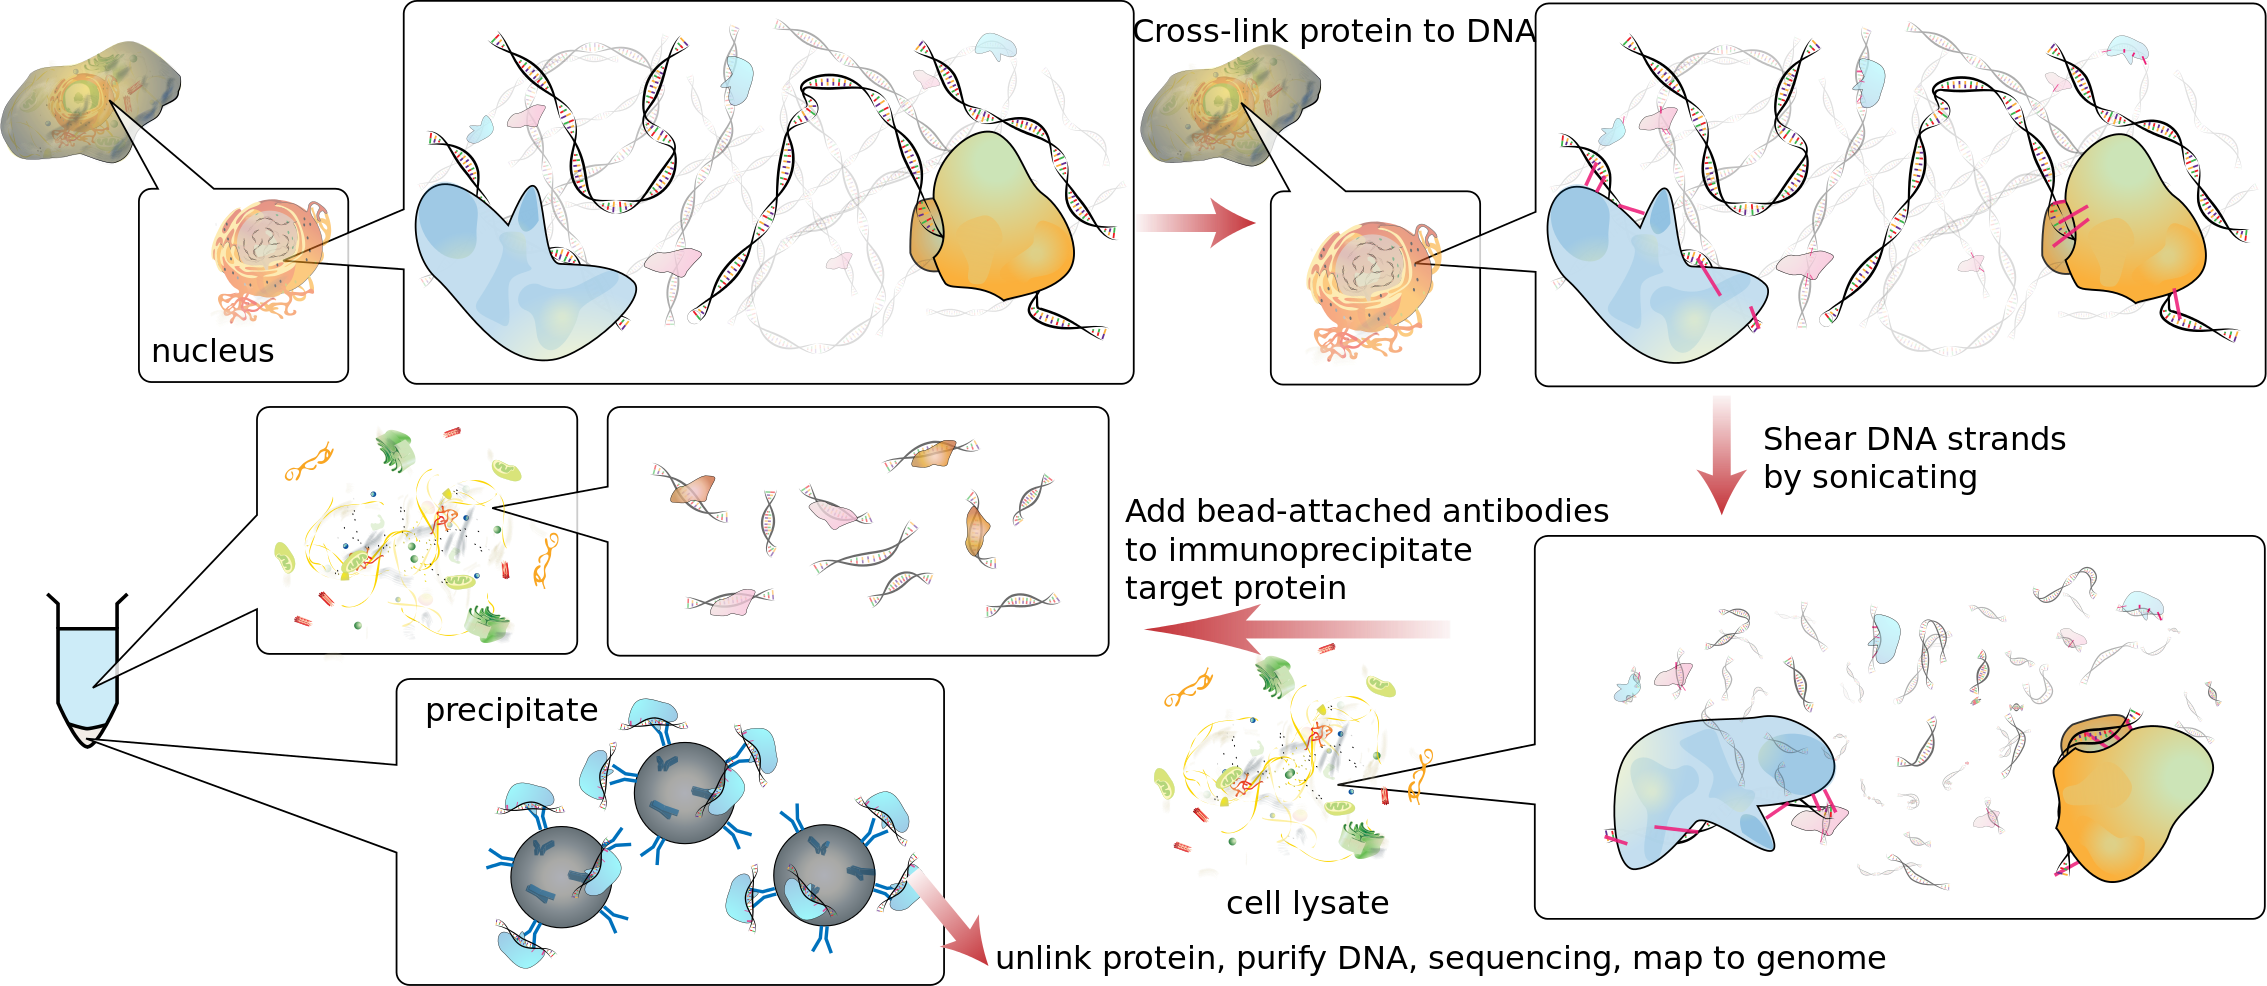
\includegraphics[width=\textwidth]{Chromatin_immunoprecipitation_sequencing_wide.png}

  Source: ``ChIP-sequencing,'' Wikipedia.
\end{frame}

\begin{frame}
  \frametitle{Problem: inaccurate unsupervised peak predictions}
  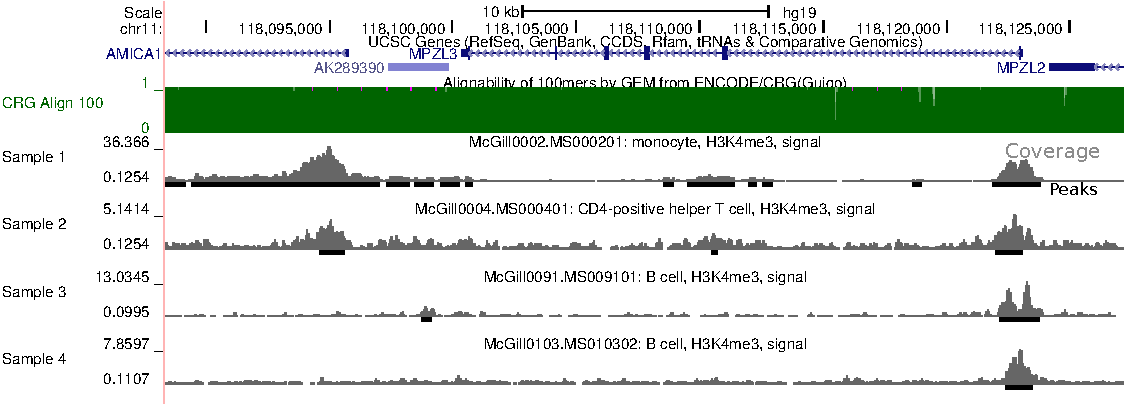
\includegraphics[width=\textwidth]{screenshot-ucsc-edited}

  Grey profiles are normalized aligned read count signals.

  Black bars are ``peaks'' called by MACS2 (Zhang {\it et al.}, 2008):
  \begin{itemize}
  \item many false positives (sometimes false negatives as well).
  \item overlapping peaks have different start/end positions.
  \end{itemize}
\end{frame}

% \begin{frame}
%   \frametitle{Previous work in genomic peak detection}
%   \begin{itemize}
%   \item Model-based analysis of ChIP-Seq (MACS), Zhang et al, 2008.
%   \item SICER, Zang et al, 2009.
%   \item HOMER, Heinz et al, 2010.
%   \item CCAT, Xu et al, 2010.
%   \item RSEG, Song et al, 2011.
%   \item Triform, Kornacker et al, 2012.
%   \item Histone modifications in cancer (HMCan), Ashoor et al, 2013.
%   \item PeakSeg, Hocking, Rigaill, Bourque, ICML 2015.
%   \item PeakSegJoint Hocking and Bourque, arXiv:1506.01286.
%   \item ... dozens of others.
%   \end{itemize}
%   Two big questions: how to choose the best...
%   \begin{itemize}
%   \item ...algorithm? (testing)
%   \item ...parameters? (training)
%   \end{itemize}
% \end{frame}

\begin{frame}[fragile]
  \frametitle{How to choose parameters of unsupervised peak
    detectors?}
\scriptsize
19 parameters for Model-based analysis of ChIP-Seq (MACS), Zhang {\it et al.}, 2008.
\begin{verbatim}
  [-g GSIZE]
  [-s TSIZE] [--bw BW] [-m MFOLD MFOLD] [--fix-bimodal]
  [--nomodel] [--extsize EXTSIZE | --shiftsize SHIFTSIZE]
  [-q QVALUE | -p PVALUE | -F FOLDENRICHMENT] [--to-large]
  [--down-sample] [--seed SEED] [--nolambda]
  [--slocal SMALLLOCAL] [--llocal LARGELOCAL]
  [--shift-control] [--half-ext] [--broad]
  [--broad-cutoff BROADCUTOFF] [--call-summits]
\end{verbatim}
10 parameters for Histone modifications in cancer (HMCan),
Ashoor {\it et al.}, 2013.
\begin{verbatim}
minLength 145
medLength 150
maxLength 155
smallBinLength 50
largeBinLength 100000
pvalueThreshold 0.01
mergeDistance 200
iterationThreshold 5
finalThreshold 0
maxIter 20
\end{verbatim}
\end{frame}


\begin{frame}
  \frametitle{New labeling method for peak detection in ChIP-seq data}

  H {\it et al.}, {\it Bioinformatics} 2017: choose peak model/parameters
  which minimize the number of incorrectly predicted labels.

  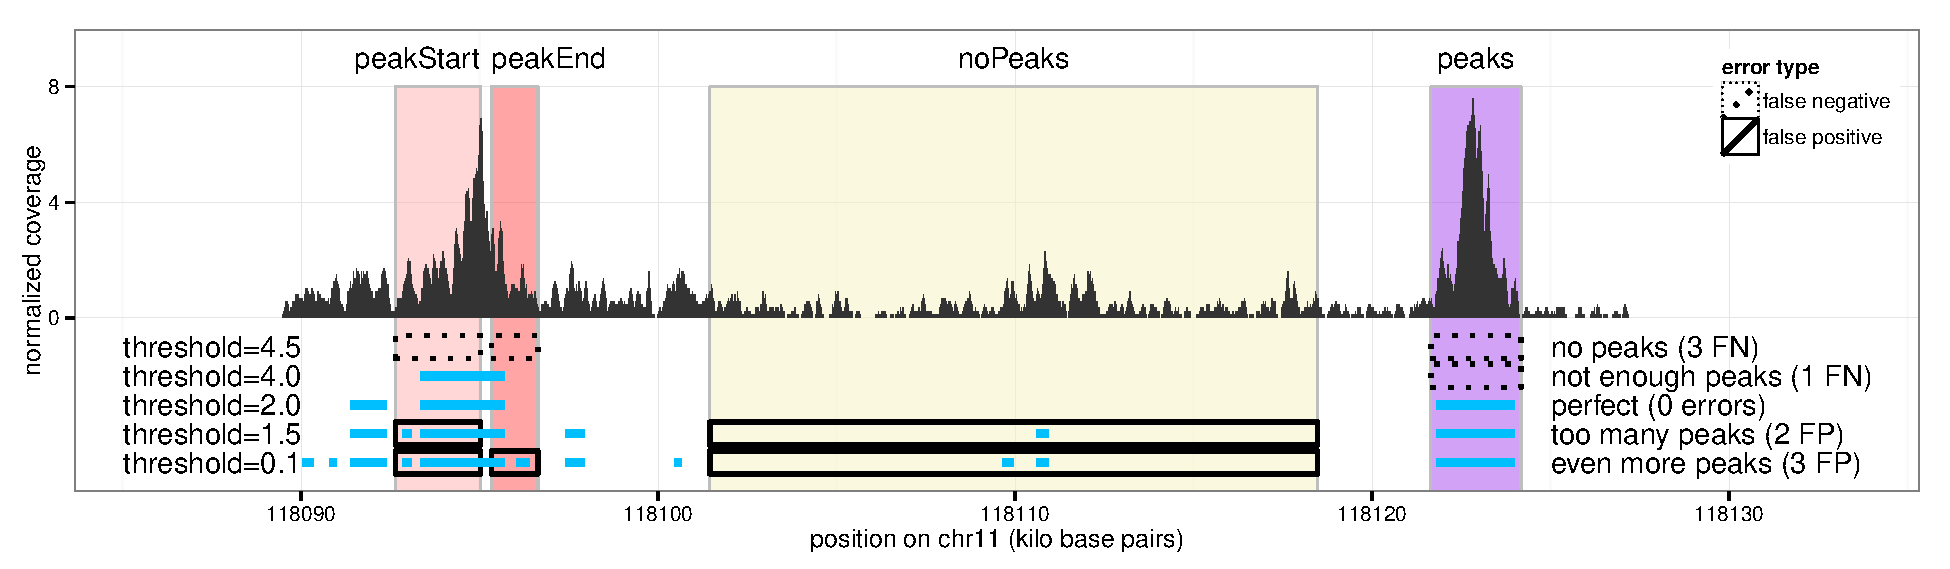
\includegraphics[width=\textwidth]{figure-PeakError.pdf}
  \begin{itemize}
  \item \textbf{peakStart}: exactly one peak start (0=FN, more=FP).
  \item \textbf{peakEnd}: exactly one peak end (0=FN, more=FP).
  \item \textbf{noPeaks}: no overlapping peaks (otherwise FP).
  \item \textbf{peakEnd}: at least one overlapping peak (otherwise FN).
  \end{itemize}
\end{frame}

\begin{frame}
  \frametitle{Two annotators provide consistent labels, but different
    precision}
  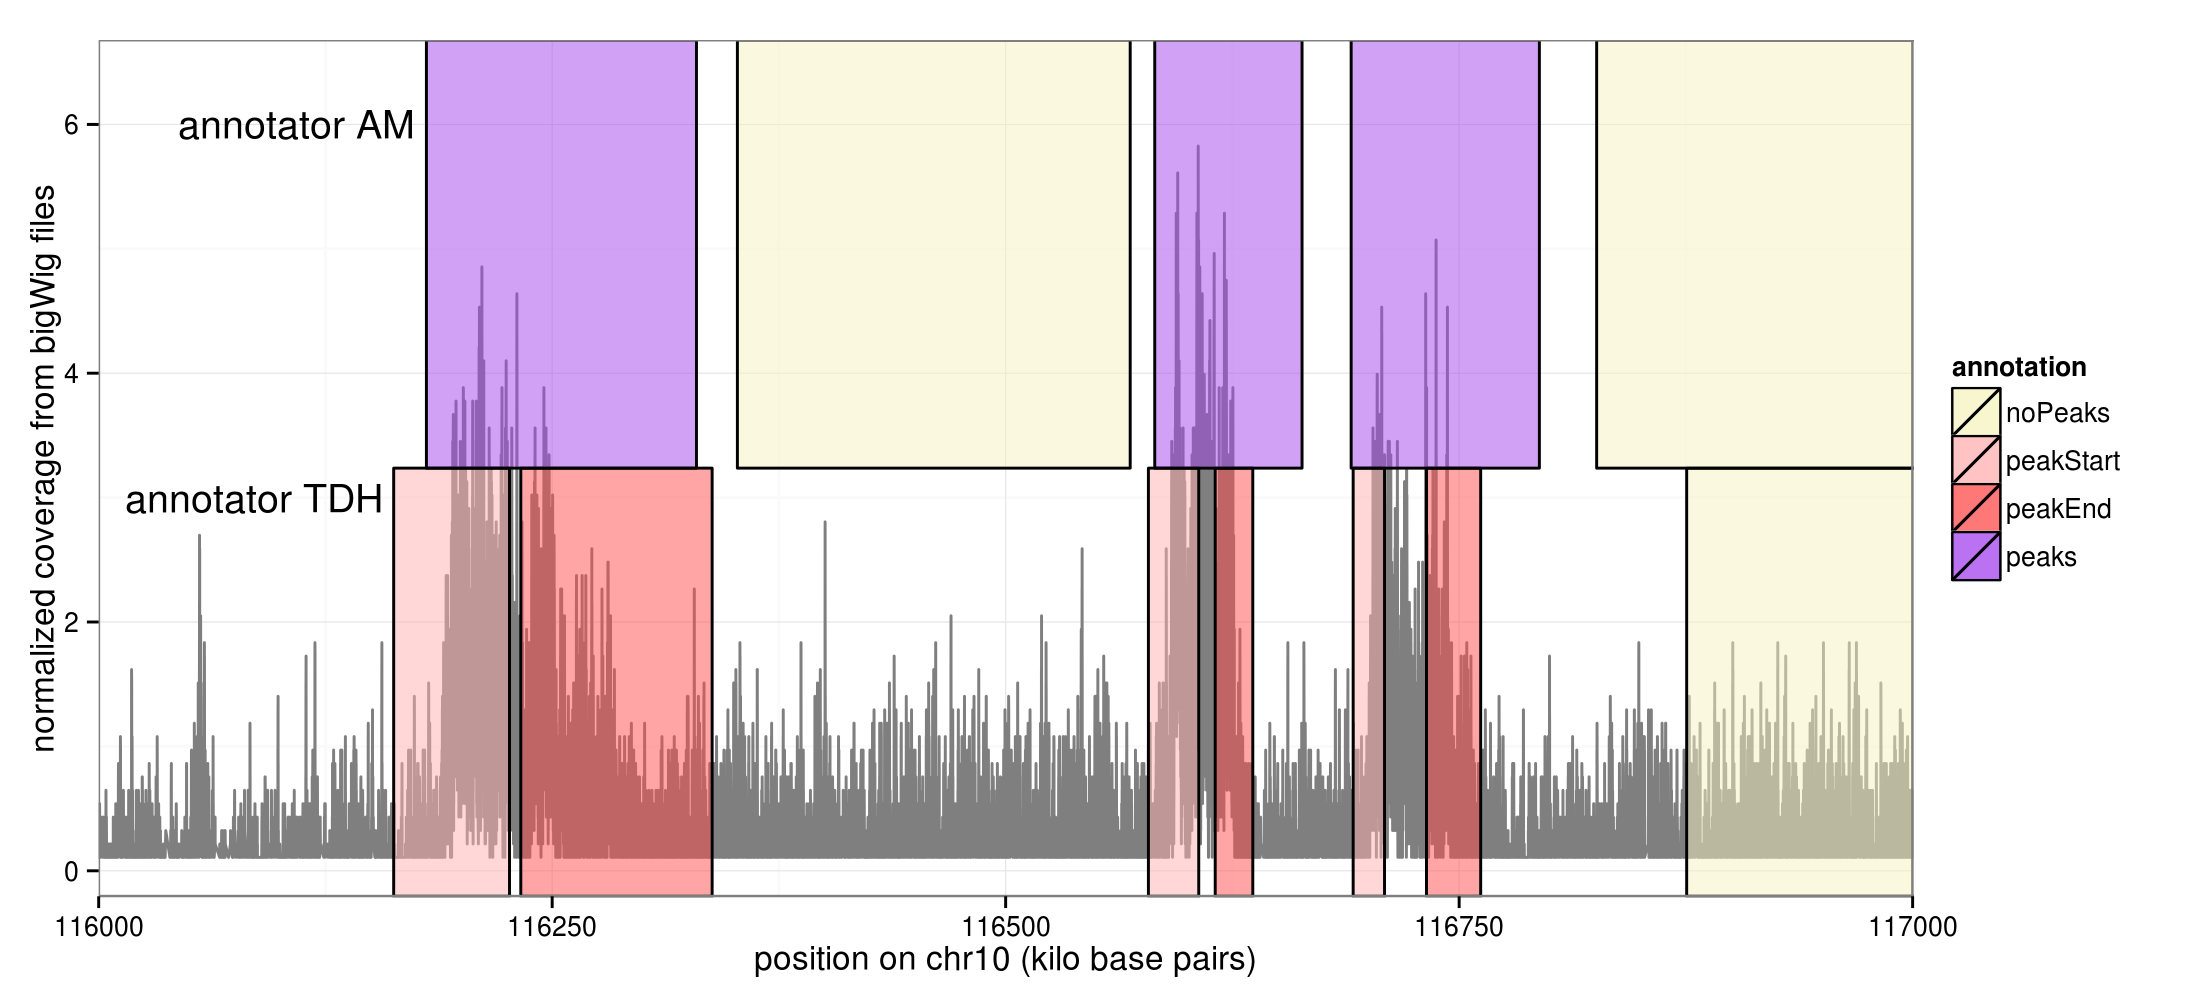
\includegraphics[width=1.1\textwidth]{screenshot-several-annotators}

  \begin{itemize}
  \item TDH peakStart/peakEnd more precise than AM peaks.
  \item AM noPeaks more precise than TDH no label.
  \end{itemize}
\end{frame}

\begin{frame}
  \frametitle{Models trained on labels from one person\\
predict accurately for another person\\
    (same histone mark and samples)}
  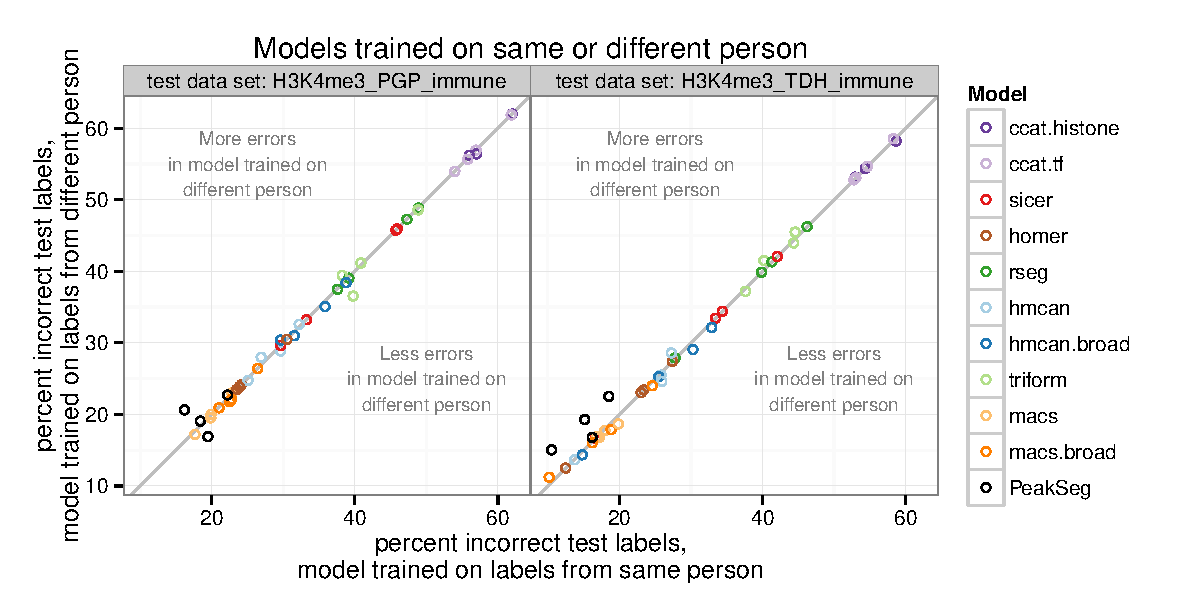
\includegraphics[width=1.1\textwidth]{figure-test-H3K4me3-annotators.pdf}

  Test error in four-fold cross-validation.
\end{frame}

\begin{frame}
  \frametitle{Only a few labels are required to train highly accurate models}
  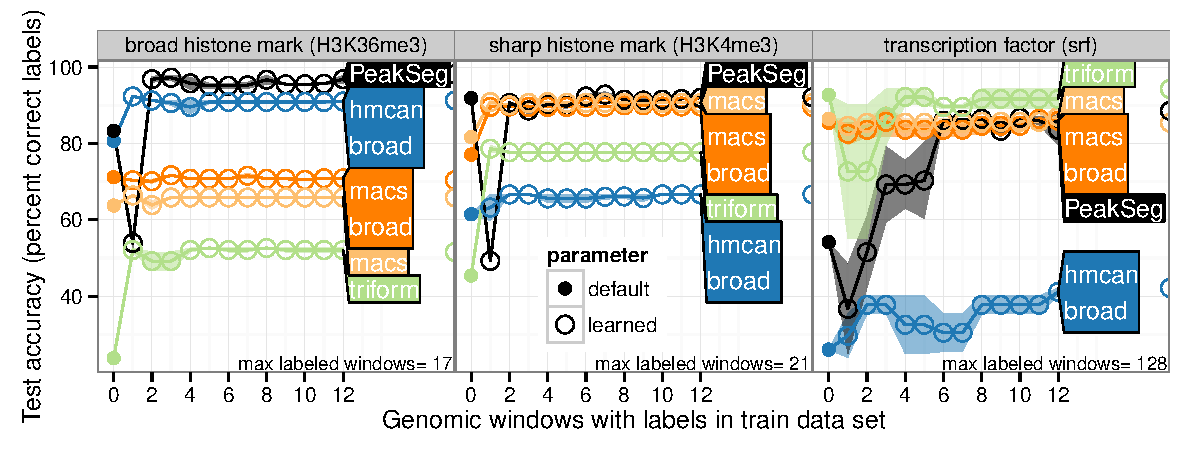
\includegraphics[width=1.1\textwidth]{figure-test-error-decreases-mean.pdf}
\end{frame}

\section{LEARNING THE PENALTY}

\begin{frame}
  \frametitle{Supervised learning algorithm for breakpoint detection}
  H {\it et al.}, {\it ICML} 2013.
  \begin{itemize}
  \item New method for learning multi-feature linear penalty
    functions in maximum likehood changepoint models.
  \item Previous work: AIC/BIC/mBIC/etc (0 learned parameters)
    and scalar penalties (1 learned parameter).
  \item Contribution: convex optimization problem and learning
    algorithm for regression with censored outputs
    $(\underline L_i, \overline L_i)$.
  \item Results: improves breakpoint detection accuracy (K-fold
    cross-validation experiments).
  \end{itemize}
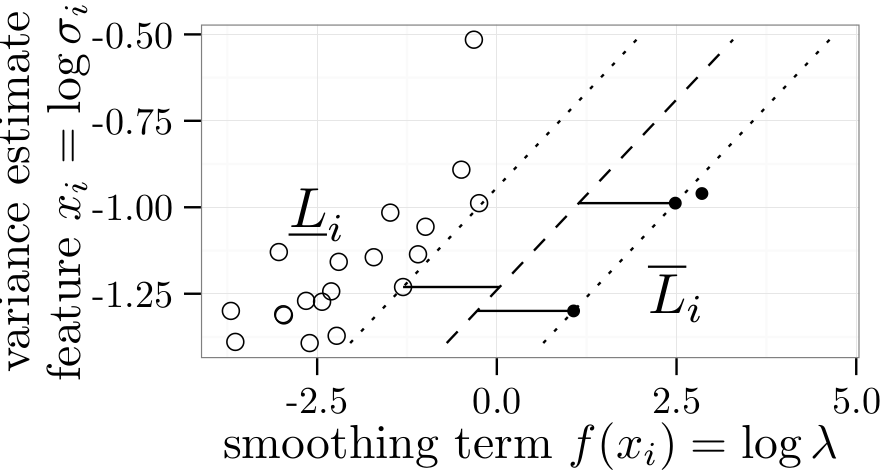
\includegraphics[width=0.4\textwidth]{screenshot-mmir-crop}
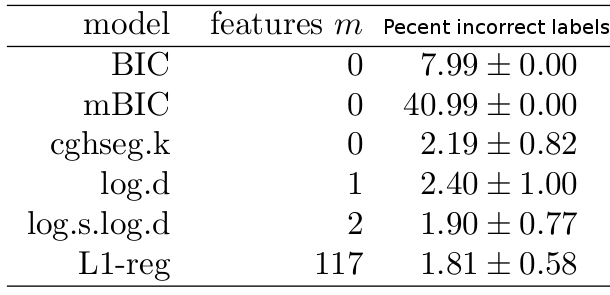
\includegraphics[width=0.4\textwidth]{screenshot-mmir-test-error}
\end{frame}

\begin{frame}
  \frametitle{useR2017 tutorial}
  
\end{frame}

\begin{frame}
  \frametitle{Nonlinear decision tree model}
  Drouin, Hocking, Laviolette {\it NIPS} 2017.
  \begin{itemize}
  \item Contribution: dynamic programming algorithm for learning a
    nonlinear decision tree model.
  \item Results: learns nonlinear patterns, improved
    breakpoint detection accuracy.
  \end{itemize}
%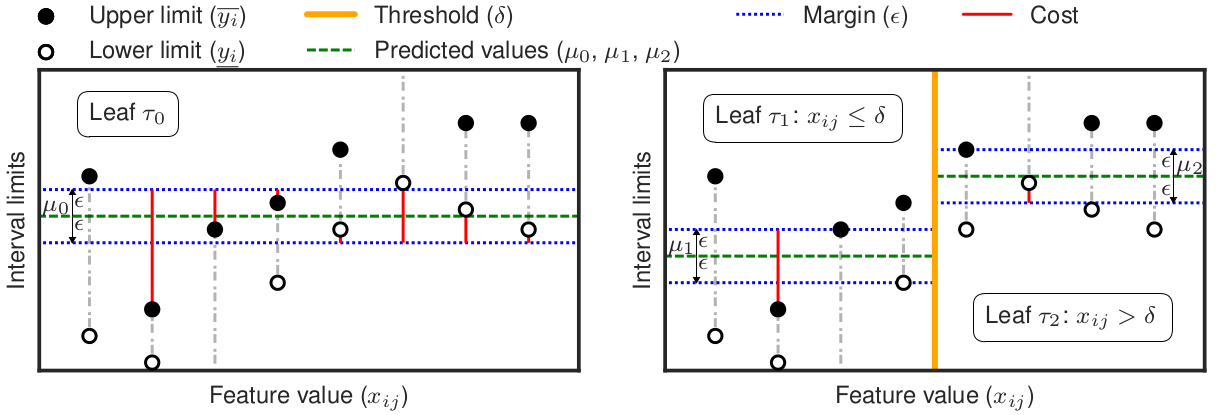
\includegraphics[width=\textwidth]{screenshot-mmit}

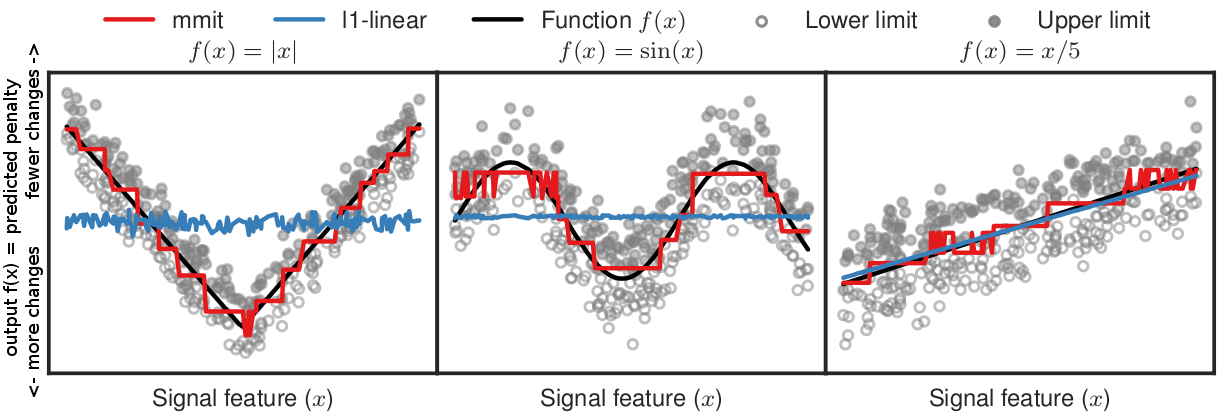
\includegraphics[width=\textwidth]{screenshot-mmit-learned}
\end{frame}

\section{OTHER PROJECTS AND FUTURE WORK}

\begin{frame}
  \frametitle{Machine learning problems in genomics}
  For example my collaborations at the McGill Genome Center:
  \begin{itemize}
  \item Predicting which people will respond to the flu vaccine based
    on SNP data. (with Maiko Narahara)
  \item Predicting which people have asthma based on SNP
    data. (with Audrey Grant)
  \item Predicting which genetic variants are pathogenic based on
    biochemistry, evolutionary conservation, etc. (with
    Najmeh Alirezaie)
  % \item Predicting genomic regions with peaks based on ChIP-seq
  %   data. (with Guillaume Bourque)
  \end{itemize}
\end{frame}

\begin{frame}
  \frametitle{Previous work limited to 
    unsupervised methods
which are neither interactive nor accurate
}
  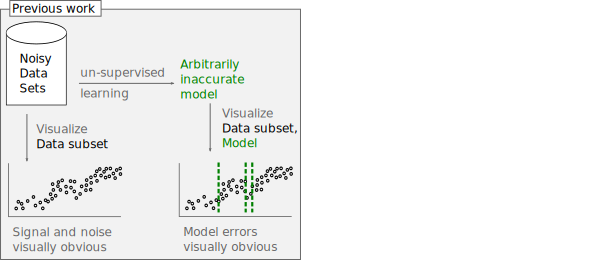
\includegraphics[height=0.5\textheight]{GenomicLearner-unsupervised.pdf}
\end{frame}

\begin{frame}
  \frametitle{GenomicLearner, an public web app for supervised interactive machine learning in genomic data}
  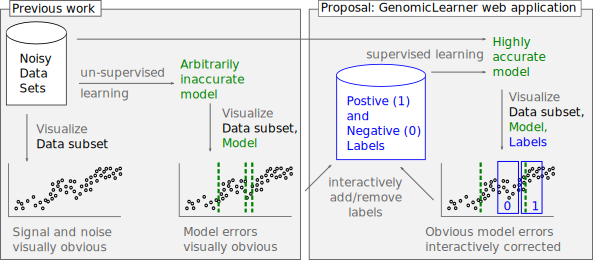
\includegraphics[height=0.5\textheight]{GenomicLearner-both.pdf}
\end{frame}


\begin{frame}
  \frametitle{Thanks for your attention!}
  Write me at \alert{\texttt{toby.hocking@mail.mcgill.ca}} to collaborate!

  \vskip 1cm

  R packages:\\
  \url{https://github.com/tdhock/PeakError}\\
  \url{https://github.com/tdhock/PeakSegJoint}

  \vskip 1cm

  Source code for slides, figures, paper online!\\
  \small
  \url{https://bitbucket.org/mugqic/chip-seq-paper}
  \vskip 1cm

  Supplementary slides appear after this one.

\end{frame}

\begin{frame}
  \frametitle{Test error in three different experiments}
  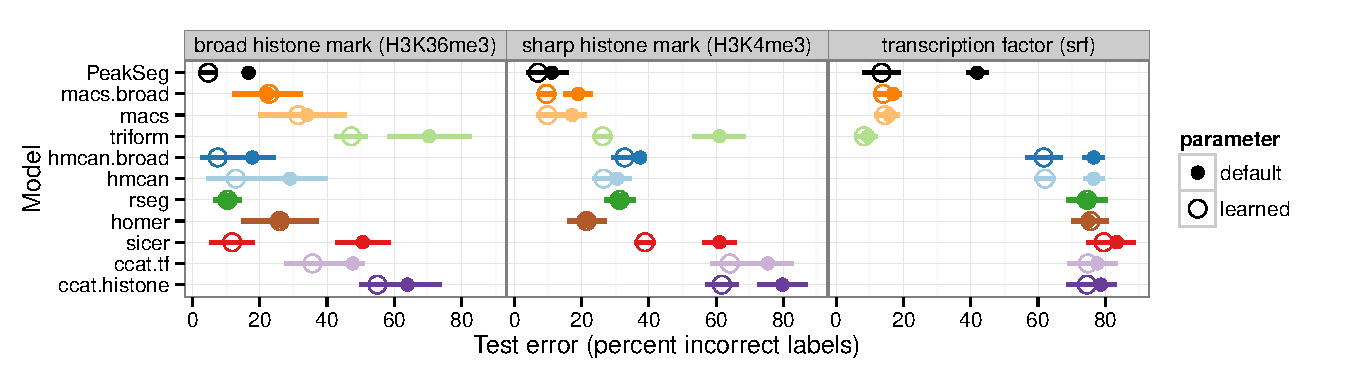
\includegraphics[width=1.1\textwidth]{figure-test-error-dots-mean.pdf}
\end{frame}

\begin{frame}
  \frametitle{Accuracy benchmark: 10 manually labeled data sets}
  \url{http://cbio.ensmp.fr/~thocking/chip-seq-chunk-db/}
  \begin{itemize}
  \item We created 12,826 labels in 7 new data sets.
  \item 4 annotators (AM, TDH, PGP, XJ).
  \item 8 cell types.
  \item 37 H3K4me3 samples (sharp peak pattern).
  \item 29 H3K36me3 samples (broad peak pattern).
  \end{itemize}
  \vskip 1cm
  \url{http://tare.medisin.ntnu.no/chipseqbenchmark/}
  \begin{itemize}
  \item 3 data sets from another group's work in 2011.
  \item 3 transcription factors: SRF, NRSF, MAX.
  \item 2 replicates per transcription factor.
  \item Different protocol: label after peak calling.
  \end{itemize}
\end{frame}

\begin{frame}
  \frametitle{Train on some samples, test on others\\
(same histone mark and person)}
  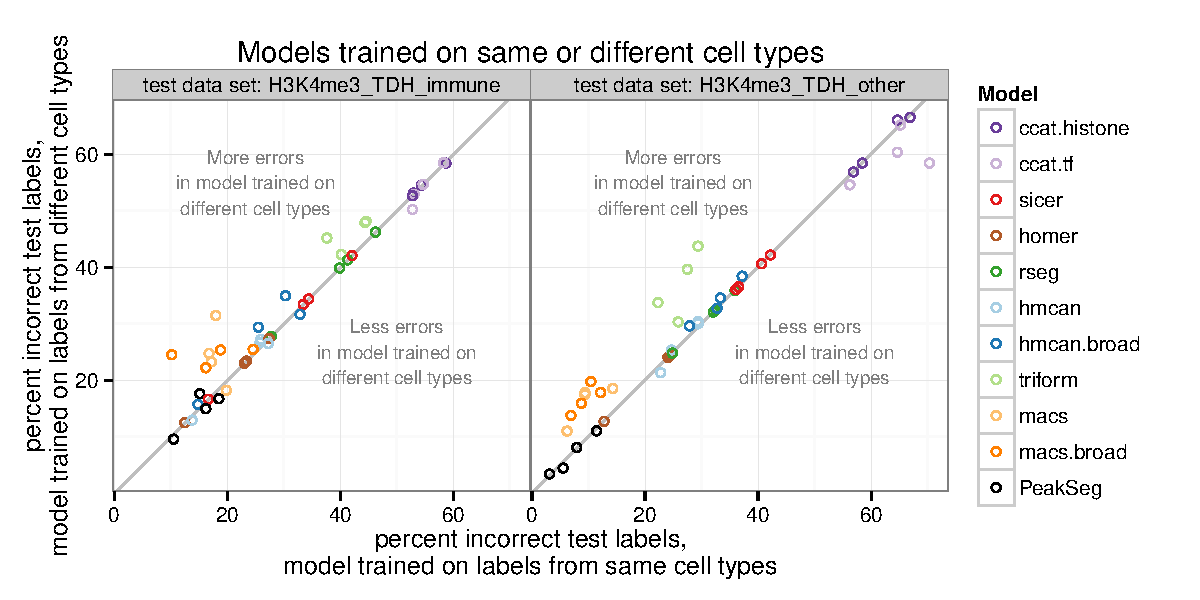
\includegraphics[width=1.1\textwidth]{figure-test-H3K4me3-types.pdf}
\end{frame}

\begin{frame}
  \frametitle{Train on one histone mark, test on another\\
(same person and samples)}
  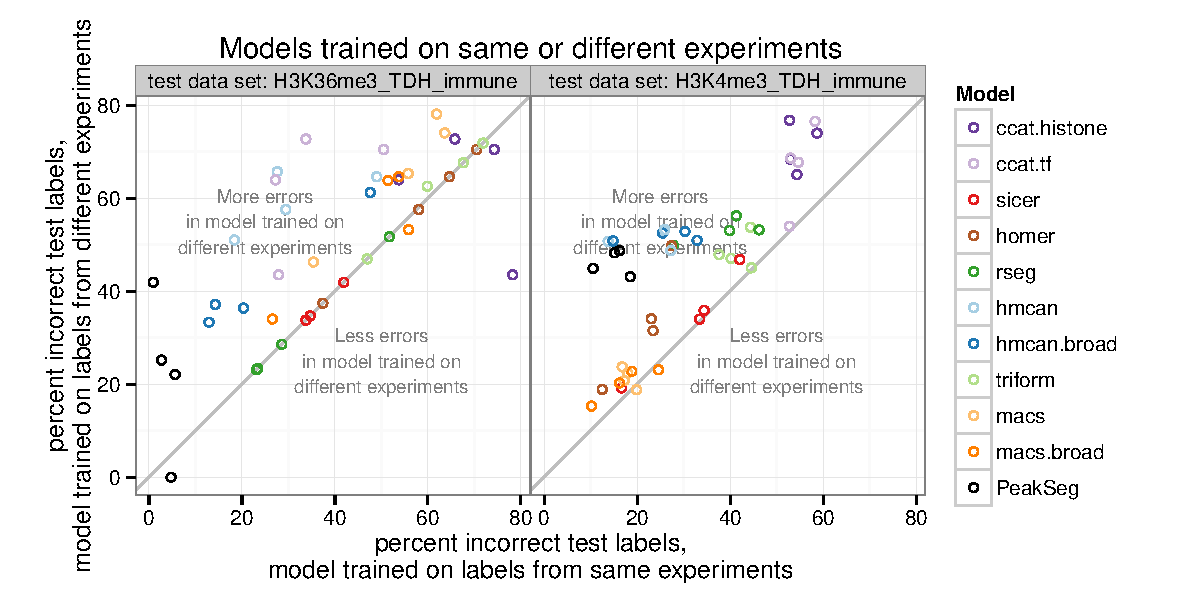
\includegraphics[width=1.1\textwidth]{figure-test-TDH-experiments.pdf}
\end{frame}


\end{document}
